
%%%%%%%%%%%%%%%%%%%%%%%%%%%%%%%%%%%%%%%%%%%%%%%%%%

%%%%%%%%%%%%%%%%% APPENDICES %%%%%%%%%%%%%%%%%%%%%

\appendix

\section{Tidal torque \& Equations of motion}
\label{app:eom}

In this appendix, we derive the equations of motion used to simulate the asteroid angular velocity during the encounter. In particular, we describe our coordinates (section \ref{sec:coordinates}) for an encountering asteroid's position and orientation, and we parametrize its density distribution via its ``density moments'' (section \ref{sec:moments}). Then we derive an arbitrary-order equation for tidal torque (section \ref{sec:tidal-torque}) and write the equations of motion for the system (section \ref{sec:eom}). We do not consider any third-body perturbations, and we assume that the body being encountered (the central body, e.g.~a planet) is much more massive than the asteroid.

\subsection{Coordinates}
\label{sec:coordinates}

We make use of two frames of reference to model this system. One is the ``inertial frame,'' with axes denoted by $\unit{X}$, $\unit{Y}$, $\unit{Z}$ and origin placed at the central body's centre of mass. $\unit{X}$ points from the central body to the asteroid periapse, and $\unit{Z}$ points parallel to the orbit angular momentum. We assume that the mass distribution of the central body is known in this inertial frame.

Our second frame is the ``body-fixed'' frame, denoted by $\unit{x}, \unit{y}, \unit{z}$. Each axis in this frame is aligned with a principal axis and rotates with the asteroid, with its origin at the asteroid's centre of mass. For definiteness, we define $\unit{z}$ to be the principal axis with maximal moment of inertia (this is the short axis mode, to use the vocabulary of Ref.~\cite{kaasalainen2001interpretation}). In general, we use capital letters to denote vectors in the inertial frame and lowercase vectors to denote vectors in the body-fixed frame.

The difference between the origins of the body-fixed and inertial frames is the position of the asteroid. We represent the relative orientations by $z-y-z$ Euler angles $\alpha$, $\beta$, and $\gamma$, such that a matrix $M$ rotating from the body-fixed to the inertial frame ($M\bm{r} = \bm{R}$) is given by
\begin{equation}
M = R_z(\alpha) R_y(\beta) R_z(\gamma).
\label{eqn:euler-angles}
\end{equation}
Here, $R_i(\theta)$ is a rotation around the unit vector $i$ by $\theta$ (figure \ref{fig:euler-angles}).

\begin{figure}
    \centering
    \begin{tikzpicture}
    \draw[-{Latex[length=3mm]}] (0, 0) -- (-4, 0) node[anchor=east] {$\unit x$};
    \draw[-{Latex[length=3mm]}] (0, 0) -- (2, -3) node[anchor=west] {$\unit y$};
    \draw[-{Latex[length=3mm]}] (0, 0) -- (0, 4) node[anchor=south] {$\unit z$};
    \draw[dashed, -{Latex[length=3mm]}] (0, 0) -- (3.7, -2) node[anchor=north] {};
    \draw[line width=0.5mm,-{Latex[length=3mm]}] (0, 0) -- (-0.5, -3) node[anchor=north] {$\unit X$};
    \draw[line width=0.5mm,-{Latex[length=3mm]}] (0, 0) -- (4, 1) node[anchor=south] {$\unit Y$};
    \draw[line width=0.5mm,-{Latex[length=3mm]}] (0, 0) -- (-1.6, 2.7) node[anchor=south] {$\unit Z$};
    \draw[->] (0.5, -0.75) arc (290:302:2.5);
    \draw (0.9, -0.9) node[anchor=center] {$\alpha$};
    \draw[->] (0, 1.2) arc (130:161:1.3);
    \draw (-0.3, 1.3) node[anchor=center] {$\beta$};
    \draw[->] (0.97, -0.52) arc (330:368:1.3);
    \draw (1.4, -0.25) node[anchor=center] {$\gamma$};
    %\draw[-{Latex[length=3mm]}] (0, 0) -- (0, 4) node[anchor=south] {$\unit Z$};
    %\draw[-{Latex[length=3mm]}] (0, 0) -- (4, 0) node[anchor=west] {$\unit Y$};
    %\draw[-{Latex[length=3mm]}] (0, 0) -- (-2, -2) node[anchor=east] {$\unit X$};
    \end{tikzpicture}
    \caption{$z-y-z$ Euler angles used in this work to express the orientation of the asteroid. Orientation is expressed as a rotation from the body-fixed axes (lowercase) to the inertial axes (bold and uppercase). The origins are co-located for demonstration purposes.}
    \label{fig:euler-angles}
\end{figure}


\subsection{Density moments}
\label{sec:moments}

In the next section, it will be shown that only certain parameters of the asteroid density distribution affect tidal torque called ``density moments.'' First, we define the un-normalized spherical harmonics $Y_{\ell m}(\theta, \phi) = P_{\ell m}(\cos \theta)e^{im\phi}$, where $P_{\ell m}$ are the associated Legendre Polynomials without the Condon-Shortley phase. The regular and irregular spherical harmonics then defined as
\begin{equation}
  \begin{split}
    S_{\ell m}(\bm r) &= (-1)^m (\ell - m)! \frac{Y_{\ell m}(\unit r)}{r^{\ell+1}} \\
    R_{\ell m} (\bm r) &= (-1)^m \frac{r^\ell}{(\ell + m)!} Y_{\ell m}(\unit r).
  \end{split}
\end{equation}
These spherical harmonics obey many useful identities summarized in Ref.~\cite{Gelderen1998TheSO}, which are also useful for quantum mechanics.

We define the density moments of an asteroid in equation \ref{eqn:klm}.
Note that these are complex. The length defined in equation \ref{eqn:am} can be thought of as akin to the radius of the asteroid (a spherical, uniform-density asteroid has radius $a_\mathcal{A}\sqrt{5/3} $). Both equations \ref{eqn:am} and \ref{eqn:klm} should be computed in the body-fixed frame.

Equations \ref{eqn:am} and \ref{eqn:klm} can be extended to the central body:
\begin{equation}
  \begin{split}
    &J_{\ell m} = \frac{1}{\mu_\mathcal{B} a_\mathcal{B}^\ell} \int_\mathcal{B} d^3 r \rho_\mathcal{B}(\bm r) R_{\ell m}(\bm r)\\
    &a_\mathcal{B}^2 = \frac{1}{\mu_\mathcal{B}} \int_\mathcal{B} d^3 r \rho_\mathcal{B}(\bm r) r^2.
  \end{split}
  \label{eqn:jlm}
\end{equation}
which should be computed in the inertial frame.

Note that both $J_{\ell m}$ and $K_{\ell m}$ are unitless. We call them ``moments'' because the $R_{\ell m}(\bm r)$ contains an $r^\ell$ dependence so that $K_{\ell m}$ is the $\ell$th density moment of the asteroid. The gravitational potential field of the asteroid can be written entirely in terms of $K_{\ell m}$ and $a_\mathcal{A}$, so we expect not to need any information about the density distribution of the asteroid beyond these parameters to compute tidal torque.

These moments share several key properties which we discuss before continuing. Firstly, for real mass density, properties of the spherical harmonics imply that $K_{\ell m} = (-1)^m K_{\ell, -m}^*$. Therefore, the set of $K_{\ell m}$ for $\ell < \ell_\text{max}$ contains $\ell_\text{max}^2$ degrees of freedom. However, some of these degrees of freedom are redundant with the choice of coordinates as we discuss next.

By definition, $K_{00}=1$. Furthermore, $K_{1m} = 0$ since the body-fixed frame is centred on the asteroid centre of mass. Further calculation reveals that the alignment of the body-fixed frame with the asteroid principal axes also forces $K_{21}= 0$ and $\Im K_{22}=0$ and the same for $m<0$. The only physical density moments for $\ell \leq 2$ are therefore $K_{22}$ and $K_{20}$, which are related to the moment of inertia around each principal axis by
\begin{equation}
  \begin{split}
    I_x &= \frac{2}{3}\mu_\mathcal{A} a_\mathcal{A}^2 \parens{K_{20} - 6 K_{22} + 1}\\
    I_y &= \frac{2}{3}\mu_\mathcal{A} a_\mathcal{A}^2 \parens{K_{20} + 6 K_{22} + 1}\\
    I_z &= \frac{2}{3}\mu_\mathcal{A} a_\mathcal{A}^2 \parens{-2K_{20} + 1}.
  \end{split}
  \label{eqn:moi}
\end{equation}
Incidentally, the definition of $a_\mathcal{A}$ was chosen to satisfy equation \ref{eqn:moi}.

The physical meaning of $K_{22}$ and $K_{20}$ can also be interpreted via a special case: if the asteroid is a uniform-density triaxial ellipsoid, the moments of inertia are simple to compute in terms of the semi-axis lengths and can be compared to those found in equation \ref{eqn:moi}. This yields semi-axis lengths of 
\begin{equation}
  \begin{split}
  a &= \sqrt{\frac{5}{3}}a_\mathcal{A}\sqrt{1-2K_{20}+12K_{22}}\\
  b &= \sqrt{\frac{5}{3}}a_\mathcal{A}\sqrt{1-2K_{20}-12K_{22}}\\
  c &= \sqrt{\frac{5}{3}}a_\mathcal{A}\sqrt{1+4K_{20}}.
  \label{eqn:ellipsoid-axes}
  \end{split}
\end{equation}

The physical meaning of the higher-order moments $K_{3m}$ can be aided by assessing their symmetry properties. An asteroid that is mirror-symmetric along the $\unit{x}$ axis (meaning $\rho_\mathcal{A}(x,y,z)=\rho_\mathcal{A}(-x,y,z)$) necessarily sets certain density moments to zero. Which density moments are zeroed by which mirror symmetries is outlined in table \ref{tab:klm-symmetries}. Note that, while no mirror symmetries set $K_{00}$, $K_{20}$, or $K_{22}$ equal to zero, mirror symmetries exist which zero all the other moments, including $K_{3m}$. $\Re K_{32}$, $K_{31}$, and $K_{30}$ are the only $K_{3m}$ components zeroed by only one axis. This will not affect our fit results for $K_{3m}$, but when we compute density moments for sample distributions, we find that most $K_{3m}=0$.

\begin{table}
  \centering
  \begin{tabular}{c|ccccccc}
    \hline
    $\ell$ & $\Re K_{\ell 3}$ & $\Im K_{\ell 3}$ & $\Re K_{\ell 2}$ & $\Im K_{\ell 2}$ & $\Re K_{\ell 1}$ & $\Im K_{\ell 1}$ & $K_{\ell 0}$ \\ \hline
    0 &  &  &  &  &  &  & -\\ 
    1 &  &  &  &  & x & y & z\\ 
    2 &  &  & - & x,y & y,z & x,z & -\\ 
    3 & x,z & y,z & z & x,y,z & x & y & z\\ \hline
  \end{tabular}
  \caption{Axes of mirror symmetry that imply zeroed density moments. For example, for mirror symmetries along $\unit y$ or $\unit z$, $\Im K_{32}=0$. Mirror symmetry along $\unit x$ means $\rho_\mathcal{A}(x, y, z) = \rho_\mathcal{A}(-x, y, z)$. Dashes indicate that none of the mirror symmetries zero the moment in question. Since $r^2>0$ for $r\neq 0$, no symmetries set $a_\mathcal{A}=0$ either.}
  \label{tab:klm-symmetries}
\end{table} 

Finally, the requirement that $\rho_\mathcal{A}(\bm r) \geq 0$ everywhere restricts $K_{\ell m}$. In the case of $K_{2m}$, this fact and the constraint that $I_z$ is larger than $I_x$ or $I_y$ requires $K_{20}$ and $K_{22}$ to fall in the triangle
\begin{equation}
  -\frac{1}{4} \leq K_{20} \leq 0, \qquad |K_{22}| \leq -\frac{K_{20}}{2}.
  \label{eqn:parameter-bounds}
\end{equation}
In practice, we also observe that $|K_{3m}| < 1$; often, $|K_{3m}| < 0.01$ even.





\subsection{Tidal torque}
\label{sec:tidal-torque}

Derivations for the tidal torque experienced by a rigid body in the gravitational field of a larger mass have been computed by several previous studies \cite{paul88,HouMar2017,BOUE2009750, ashenberg07}, often in terms of the moment of inertia of the rigid body (or higher order moments of inertia), and to varying degrees of precision. A simple, first-order derivation is also easily computable in terms of the asteroid moment of inertia in the inertial frame.

Here, we present a novel derivation of the tidal torque to arbitrary orders in terms of the density moments of an asteroid defined in section \ref{sec:moments}. These density moments can be pre-computed and do not have to be re-evaluated every time-step.

Throughout this paper, we assume that the asteroid remains rigid throughout the encounter. We also assume no third-body perturbations from other Solar System objects. (Actually, third-body perturbing objects are allowed if they are closer to the central body's centre of mass than the asteroid perigee distance. Then, their density moments can be included in the density moments of the central body and this derivation can still be used.) For the sake of simplicity, we also assume that the density moments of the central body are known and do not evolve with time (i.e., the central body's rotation is marginal compared to the timescale of the encounter).

The gravitational potential energy of the central body is, in its most general form,
\begin{equation}
V(\bm R') = -G\int_\mathcal{B} d^3 R \rho_\mathcal{B}(\bm R) \frac{1}{|\bm{R}-\bm{R'}|}.
\label{eqn:first-pe}
\end{equation}
where $\rho_\mathcal{B}$ is the density distribution of the central body and $\mathcal{B}$ indicates the central body's volume. All vectors here are written in the inertial frame. Given $|\bm{R}| < |\bm{R'}|$, Ref.~\cite{Gelderen1998TheSO} gives the identity
\begin{equation}
  \frac{1}{|\bm R - \bm R'|} = \sum_{\ell, m} R_{\ell m}(\bm R) S_{\ell m}^*(\bm R'),
  \label{eqn:ylm-expansion}
\end{equation}
where the sum is shorthand for $\sum_{\ell, m} = \sum_{\ell = 0}^\infty \sum_{m=-\ell}^\ell$.
We are interested in translating the potential energy of equation \ref{eqn:first-pe} to the body-fixed frame. To do this, we let $\bm{R'} = \bm D + \bm U$, where $\bm D$ is the location of the asteroid in the inertial frame. We further define $\bm U = M\bm u$, where $\bm u$ is in the body-fixed frame and $M$ is the rotation matrix given by the Euler angles $\alpha$, $\beta$, and $\gamma$ (see section \ref{sec:coordinates}). The translation from $\bm {R'}$ to $\bm U$ is then attained by the identity 
\begin{equation}
  S_{\ell m}(\bm R') = \sum_{\ell', m'} (-1)^{\ell'}R^*_{\ell' m'}(\bm U)S_{\ell+\ell', m + m'} (\bm D),
  \label{eqn:ylm-translation}
\end{equation}  
provided by Ref.~\cite{Gelderen1998TheSO}, and from $\bm U$ to $\bm u$ is given by
\begin{equation}
  \begin{split}
    Y_{\ell m}(M\bm u) = \sum_{m'=-\ell}^\ell & (-1)^{m+m'}\sqrt{\frac{(\ell-m')!(\ell+m)!}{(\ell+m')!(\ell-m)!}} \\
    & \times \mathcal{D}^\ell_{mm'}(M)^* Y_{\ell m'}(\bm u).\\
  \end{split}
  \label{eqn:ylm-rotation}
\end{equation}
Here, $\mathcal{D}^\ell_{mm'}(M)$ are the Wigner-$D$ matrices, which are determined by the Euler angles $\alpha$, $\beta$, and $\gamma$ of $M$.

Equations \ref{eqn:first-pe} to \ref{eqn:ylm-rotation} then provide formula for $V(\bm u)$ expressed as a sum of integrals over $\mathcal{B}$ of the central body density $\rho_\mathcal{B}(\bm R)$ times $R_{\ell m}(\bm R)$. These are expressed via equation \ref{eqn:jlm} as $J_{\ell m}$.

The tidal torque experienced by the asteroid (in the body-fixed frame) is given by
\begin{equation}
  \bm{\tau}(\bm u) = \int_\mathcal{A} d^3 u \rho_\mathcal{A}(\bm u) (\bm u \times (-\nabla_{\bm u} V(\bm u)))
\end{equation}
where $\rho_\mathcal{A}$ is the density distribution of the asteroid and $\mathcal{A}$ indicates the volume of the asteroid. Making use of one more identity concerning the derivatives of spherical harmonics:
\begin{equation}
  \begin{split}
  \bm u \times \nabla R_{\ell m}(\bm u)=&\frac{1}{2}\Big[(i\unit x - \unit y)(\ell-m+1)R_{\ell,m-1}(\bm u)\\
  &+(i\unit x+\unit y)(\ell+m+1)R_{\ell,m+1}(\bm u)\\
  & +2im\unit z R_{\ell m}(\bm u)\Big],
  \end{split}
\end{equation}
tidal torque can now be expressed as a function only of $J_{\ell m}$, $K_{\ell m}$, $a_\mathcal{A}$, $a_\mathcal{B}$, and the asteroid orientation and position. This equation is given explicitly as equation \ref{eqn:tidal-torque}. Some $K_{\ell m}$ terms are written in this equation with $|m|>\ell$; these should all be taken to be zero.

Equation \ref{eqn:tidal-torque} possesses a few explicit properties which we discuss before writing the asteroid equations of motion. Firstly, $K_{00}$ does not appear, so that $\bm \tau$ is independent of asteroid mass. The mean density of the asteroid is therefore not constrained by tidal torque analysis. Secondly, torque is largest when $D$ is small (as expected), with the leading order of $\bm \tau$ proportional to $D^{-3}$. Thirdly, each $J_{\ell m}K_{\ell' m'}$ term is multiplied by $(a_\mathcal{B}/D)^\ell (a_\mathcal{A}/D)^{\ell'}$, the latter of which especially is small in most cases. Equation \ref{eqn:tidal-torque} can therefore be computed approximately by removing terms of large $\ell$ and $\ell'$. For our analysis, we removed $\ell' > 3$ and we usually keep only $\ell=0$. Note that $\ell=1$ contributes nothing since $J_{1m}=0$.

Further insight can be gained by remarking the value of the first-order of $\bm \tau$ for particular Euler angle cases. Setting $\beta = 0$ produces diagonal Wigner-$D$ matrices, and hence $\bm \tau \parallel \unit z$ to first-order. Also, the component $\tau_z$ oscillates, so that for certain values of $\alpha$ and $\gamma$, $\bm \tau = 0.$ This $\beta=0$ condition is equivalent to $\unit z \parallel \unit Z$ (see figure \ref{fig:euler-angles}).

For $\beta = \pi/2$, there are two interesting cases. One is for $\alpha = \phi$ (or $\alpha = \pi + \phi$), where $\phi$ is the angle between the asteroid and the perigee. In this case, $\tau = 0$ to first-order. The second case is $\alpha = \phi \pm \pi/2$, when again $\bm \tau \parallel \unit z$ and $\tau_z$ oscillates. At perigee ($\phi=0$), these conditions are equivalent to $\unit z \parallel \unit X$ and $\unit z \parallel \unit Y$ respectively.

The $\bm \tau \parallel \unit z$ cases are interesting because they do not induce tumbling. If velocity is $\bm \omega \parallel \unit z$ (a non-tumbling state, since $\unit z$ is a principal axis), then $\bm \omega \parallel \bm L$ and $\bm \tau = \dot{\bm L} \parallel \dot{\bm \omega}$ so that $\bm \omega$ remains parallel to $\unit z$ and non-tumbling. These cases of torque are additionally significant because not as many terms contribute to $\tau_z$ as to $\tau_x$ and $\tau_y$.

\subsection{Equations of motion}
\label{sec:eom}


The equations of motion of the asteroid position $\bm D$ are given by Newton's law of gravitation:
\begin{equation}
  \dot{\bm V} = -\frac{G \mu_\mathcal{B}}{D^3} \bm D \qquad \dot{\bm D} = \bm V
  \label{eqn:pos-eom}
\end{equation}
Rather than derive equations of motion for the Euler angles (which suffer from gimbal lock), we instead represent the orientation of the asteroid with a quaternion $\quat q$ which can be converted into Euler angles to compute $\mathcal{D}(\alpha, \beta, \gamma)$. This quaternion evolves as 
\begin{equation}
  \dot{\quat q} = \frac{1}{2}\quat q\quat \omega.
  \label{eqn:quat-eom}
\end{equation}
for angular velocity $\bm \omega$ given in the body-fixed frame. The equations of motion of $\bm \omega$ in turn are given by
\begin{equation}
  \begin{split}
    I_x \dot \omega_1 - \omega_y \omega_z (I_y - I_z) &= \tau_x\\
    I_y \dot \omega_2 - \omega_z \omega_x (I_z - I_x) &= \tau_y\\
    I_z \dot \omega_3 - \omega_x \omega_y (I_x - I_y) &= \tau_z.
  \end{split}
  \label{eqn:omega-eom}
\end{equation}
Equations \ref{eqn:tidal-torque} to \ref{eqn:omega-eom} form a set of non-linear, first-order coupled differential equations in which can be numerically integrated. They are expressed in terms of the constant physical parameters $\mu_{M/m}$, $a_{M/m}$, $J_{\ell m}$ and $K_{\ell m}$ given the density moment-moment of inertia relations given by equation \ref{eqn:moi}.

Note that equation \ref{eqn:omega-eom} is independent of $a_\mathcal{A}$ to first-order in $\bm \tau$, because $I_{j} \propto a_\mathcal{A}^2$ for all $j$ and $\bm \tau \propto a_\mathcal{A}^2$. Therefore, scaling $a_\mathcal{A}$ merely scales the value of the sub-leading-order contributions to $\bm \tau$.




\section{Reference asteroid configurations}
\label{app:reference-configs}

Except when otherwise mentioned, we use the following asteroid encounter parameters. Many of the parameter choices are made to maximize the quality of observations (a close orbit, large asteroid, etc.) This is so that our uncertainties have room to grow; if the reference asteroid has low uncertainty, we would not be able to measure uncertainty increases as well when the encounter parameters are adjusted.

\begin{enumerate}
  \item An orbit around a spherical, Moonless Earth with $6$ km s$^{-1}$ excess velocity and perigee at 5 Earth radii. This orbit was chosen to roughly match that of 99942 Apophis \cite{giorgini2005recent, giorgini2008predicting, smalley20052004}, discovered on June 19, 2004 by R. A. Tucker, D. J. Tholen, and F. Bernardi. These orbital parameters correspond to an eccentricity of 3.88. The comparison to Apophis is complicated by the fact that Apophis is smaller than our $a_\mathcal{A}$ value, is tumbling \cite{PRAVEC201448}, and may change slightly in physical properties due to tidal interaction during the encounter \cite{yu2014numerical,hirabayashi2021finite}. It therefore is not entirely comparable to our analysis. 
  \item An initial roll of $\gamma_0=\pi/8$.
  \item A cadence of 2 minutes and observational uncertainty of $\sigma_\theta = 0.01$ and $\sigma_\rho / \sigma_\theta = 10^{-5}$.
  \item A rotational period of 9 hours, with the angular velocity vector distributed between the $\unit X$, $\unit Y$, and $\unit Z$ axes in a $1:2:-2$ ratio.
  \item An asteroid with radius $a_\mathcal{A} = 1$ km and $K_{3m}=0$. For $K_{22}$ and $K_{20}$, we use two standard values: one with $(K_{22}, K_{20}) = (0, -0.097)$ and one with $(0.052, -0.202)$. Including the third point obtained by reflection $K_{22}\rightarrow -K_{22}$, these are the three points that minimize the mean distance between an arbitrary point in the allowed parameter space (equation \ref{eqn:parameter-bounds}) and these reference values. The first point is called the symmetric case because the corresponding uniform-density-ellipsoid model is rotationally symmetric around $\unit z$. The second case and its reflection are called the asymmetric cases. Values of $(0.052, -0.202)$ have $a < b$ in the ellipsoid model, and the reflected value has $a > b$. If not specified, we use the $a < b$ case. Specifically, the asymmetric case has $a=1140$ m, $b=1839$ m, and $c=565$ m, while the symmetric case has $a=b=1411$ m and $c=1008$ m.
\end{enumerate}

The surface of a spherical asteroid with this rotational period and $a_\mathcal{A}$ rotates at $\SI{25}{\centi\meter\per\second}$ at the equator. The asymmetric and symmetric ellipsoids have maximum equatorial velocities of $\SI{36}{\centi\meter\per\second}$ and $\SI{27}{\centi\meter\per\second}$ respectively.

We use the asymmetric ellipsoid in nearly all runs, due to the degeneracy induced in our model when $K_{22} = 0$.



\section{The cadence cut-off}
\label{app:cadence-tests}

In section \ref{sec:scan-cadence}, we noted that posterior uncertainty as a function of observation cadence $\Delta t$ appears to increase suddenly near $\Delta t \sim T_\text{cad}=30-40$ min. In the left panel of figure \ref{fig:cad-contour}, we display contour plots of posterior uncertainty $\sigma(K_{\ell m})$ of the fit parameters as a function of both cadence $\Delta t$ and $P_\omega$ (left panel) or the relative orbit speed $t_\text{spin} / t_\text{orbit}$ (right panel). Both panels show the sudden increase in posterior uncertainty we named $T_\text{cad}$. Now $T_\text{cad}$ is visible as a function of frequency and relative orbit speed. In all cases, the value of $\gamma_0$ was set so that all data points achieve the same value of $\gamma$ at perigee.

\begin{figure*}
  \centering
  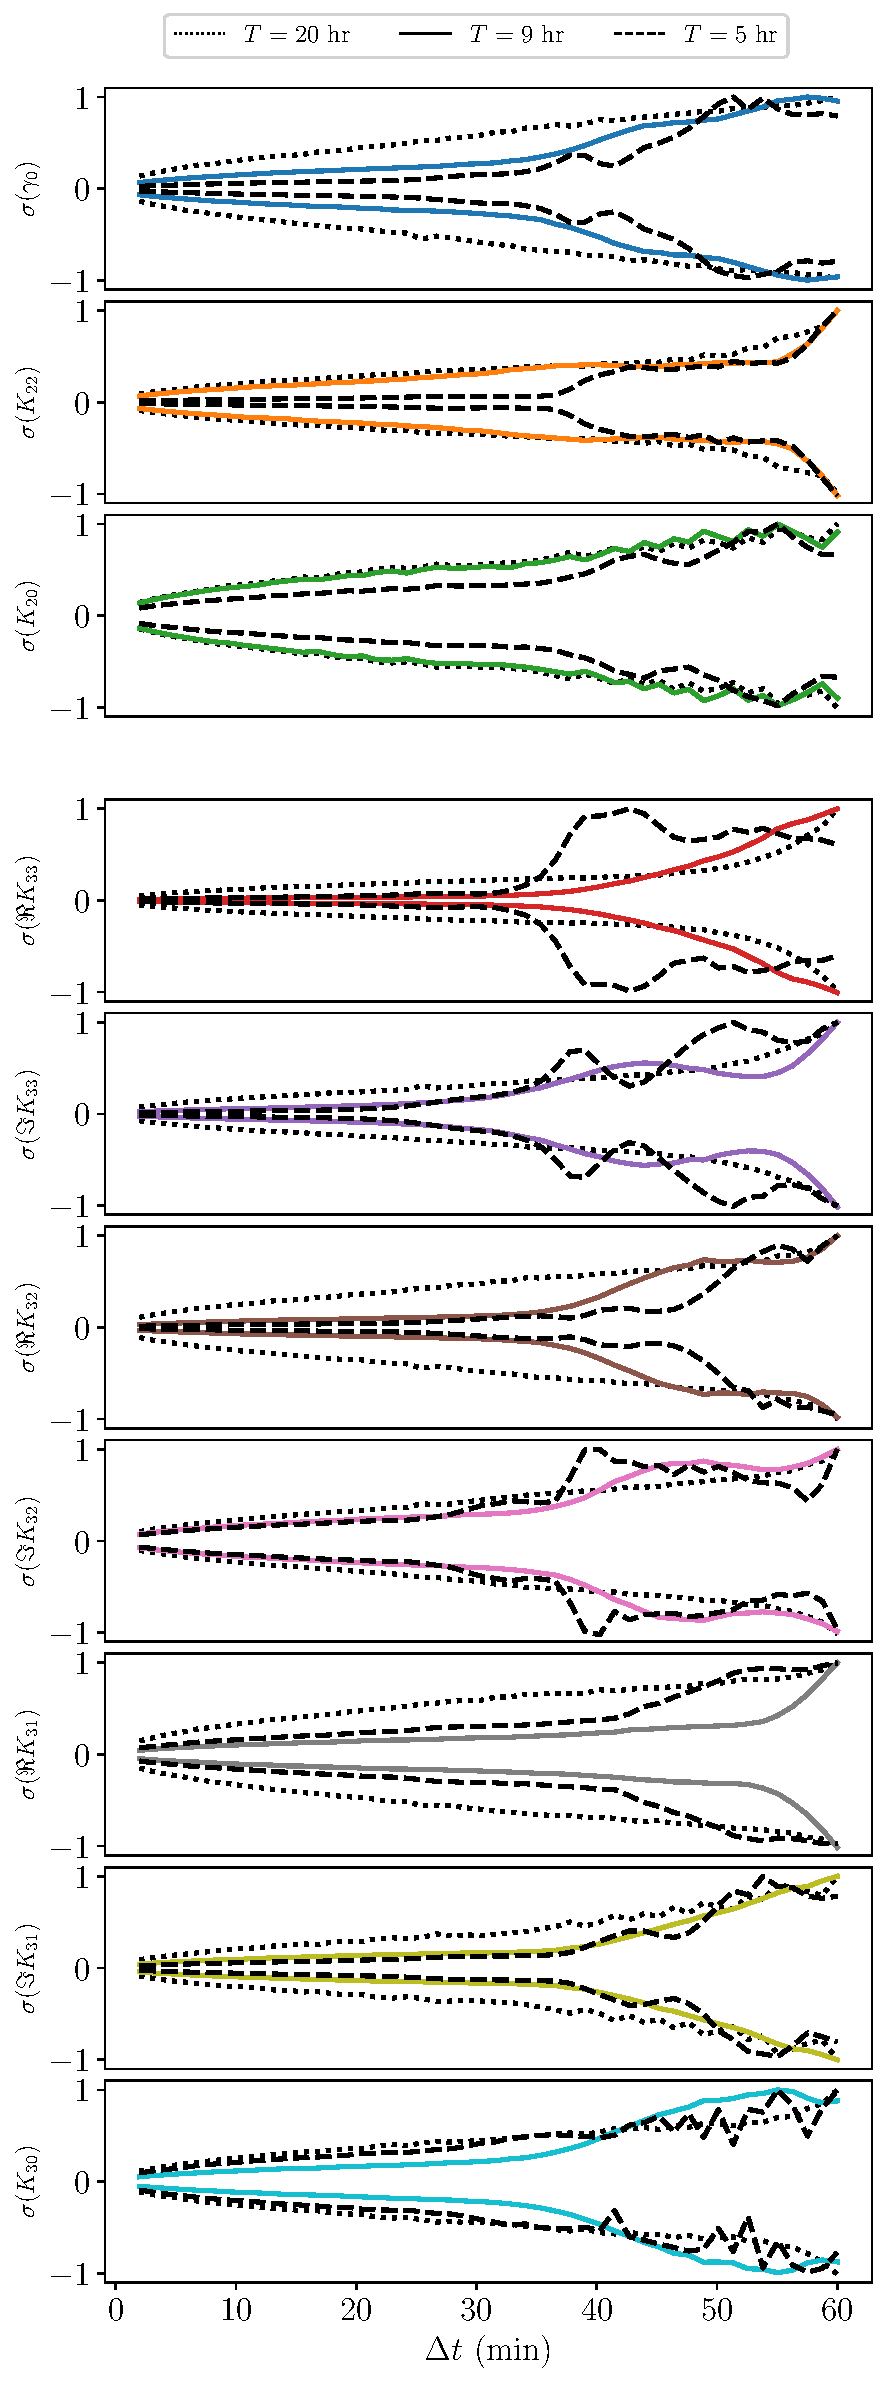
\includegraphics[width=0.49\textwidth]{figs/cad-period.pdf}\hfill
  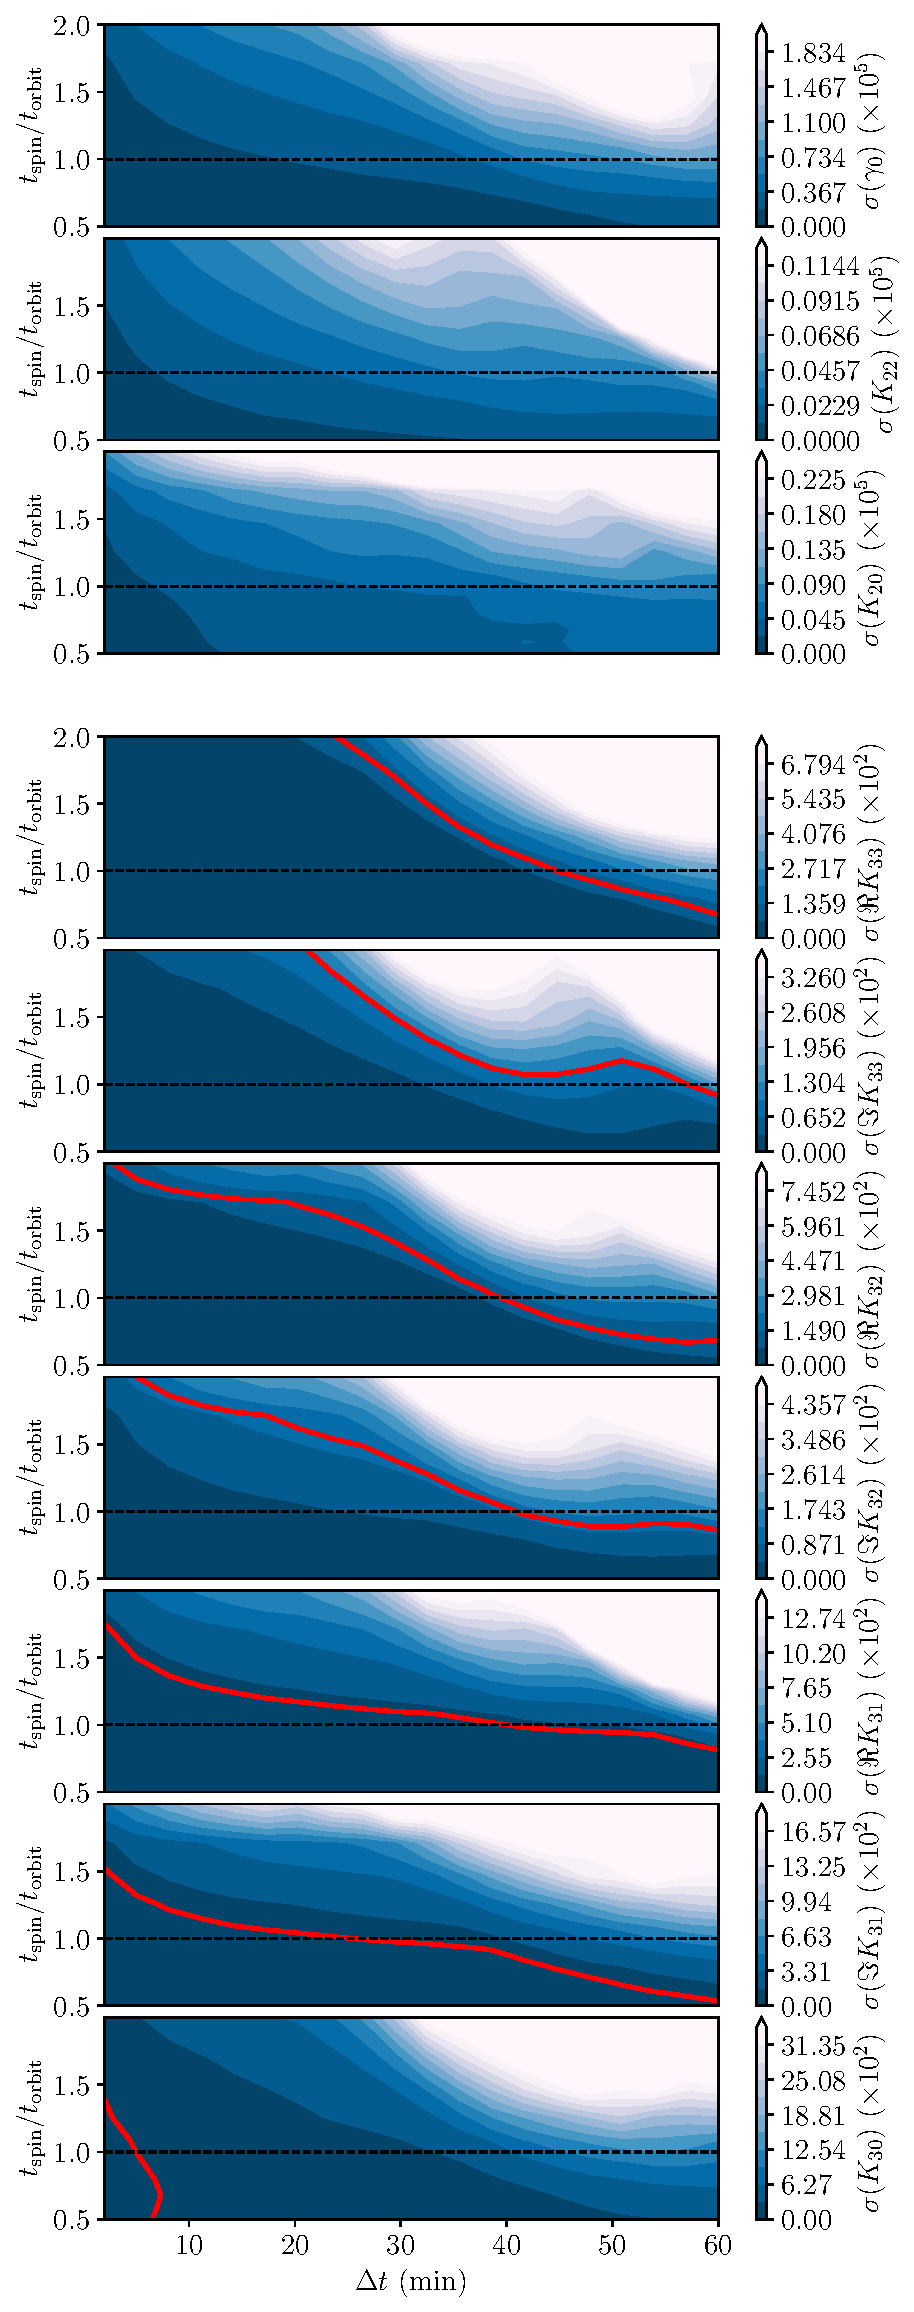
\includegraphics[width=0.49\textwidth]{figs/cad-speed.pdf}
  \caption{Contour plots showing posterior uncertainties in the first- and second-order fit parameters as a function of cadence $\Delta t$ and dynamical time scales for the encounter: rotational period $P_\omega$ (\textit{left}) and the relative speed of the orbit (\textit{right}; see text for a definition). The reference values of $P_\omega=9$ hr and $t_\text{spin}/t_\text{orbit}=1$ are shown as dotted lines. The line }
  \label{fig:cad-contour}
\end{figure*}

The relative orbit speed $t_\text{spin} / t_\text{orbit}$ was determined by un-physically increasing or decreasing the time at which the asteroid moved through the orbit determined by the equations of motion (but leaving the orbit shape unchanged). The equations of motion affecting the orientation and spin of the asteroid however were unaffected. With this unphysical process, we isolate the effect of the amount of time spent near perigee on posterior uncertainty, without inheriting additional affects that would have been caused by the orbit changing shape.

Figure \ref{fig:cad-contour} demonstrates that, near the reference values of $P_\text{omega}$ and $t_\text{spin} / t_\text{orbit}$, $T_\text{cad}$ depends on both time scales $P_\omega$ and $t_\text{spin} / t_\text{orbit}$. Specifically, high rotational period and slow orbits are optimal for large $T_\text{cad}$. The dependence on $P_\omega$ agrees with the fact that large rotational periods for fixed cadence lead to better posterior uncertainty, discussed in section \ref{sec:scan-period}. The figure also demonstrates that for large $P_\omega$, $T_\text{cad}$ depends less strongly on $P_\text{omega}$ and may even reverse its dependence such that increasing $P_\text{omega}$ decreases $T_\text{omega}$. In all cases except $\Re K_{33}$, at least constant-$\sigma(K_{\ell m})$ contour is seen to curve back such that $\Delta t$ decreases as a function of $P_\text{omega}$ for large $P_\text{omega}$. However, in these regions the cadence cut-off also dulls, as shown by the spreading of the constant-$\sigma(K_{\ell m})$ contours in this region.

The right panel of figure \ref{fig:cad-contour} shows a slightly stronger and more monotonic dependence of $T_\text{cad}$ on $t_\text{spin} / t_\text{orbit}$. It appears that slightly slower orbits sharply increases $T_\text{cad}$. Similar in the $P_\omega$ case, for increasingly fast orbits, $T_\text{cad}$ depends less on $t_\text{spin}/ t_\text{orbit}$. 
\jtd{I wanted to talk to Julien about the interpretation of this panel. Because $t_\text{spin} / t_\text{orbit}$, I find it hard to interpret. Maybe a different type of scan is better.}

Figure \ref{fig:cad-contour} demonstrates that, for large period, the cadence cut-off $T_\text{cad}$ reduces in prominence and rises to above one hour, meaning that large gaps of time between observations can still lead to well-constrained parameters in these cases. Faster orbits also lead to $T_\text{cad} > 1$ hr for for as small a decrease as $t_\text{spin} / t_\text{orbit}  \approx 75$\%.


  

\section{Computing asteroid shape from density moments}
\label{app:find-surface}

\begin{figure*}
  \centering
  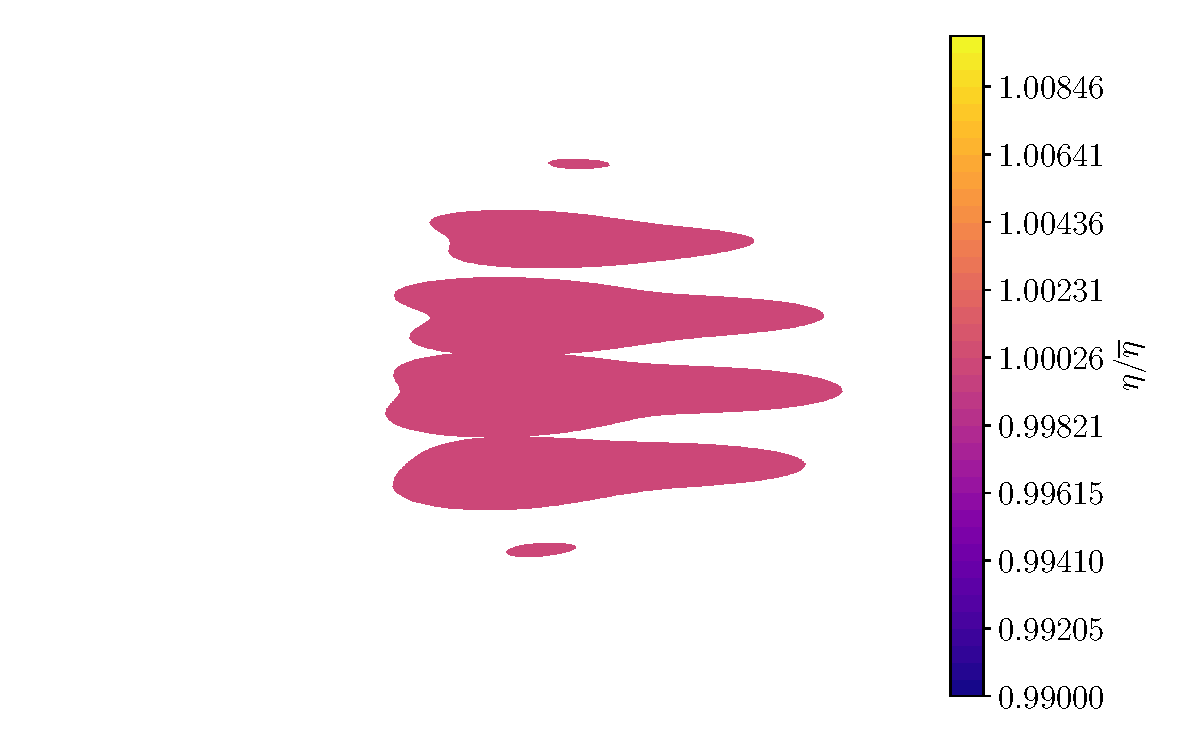
\includegraphics[width=0.45\textwidth]{figs/high-surface.pdf}\hfill
  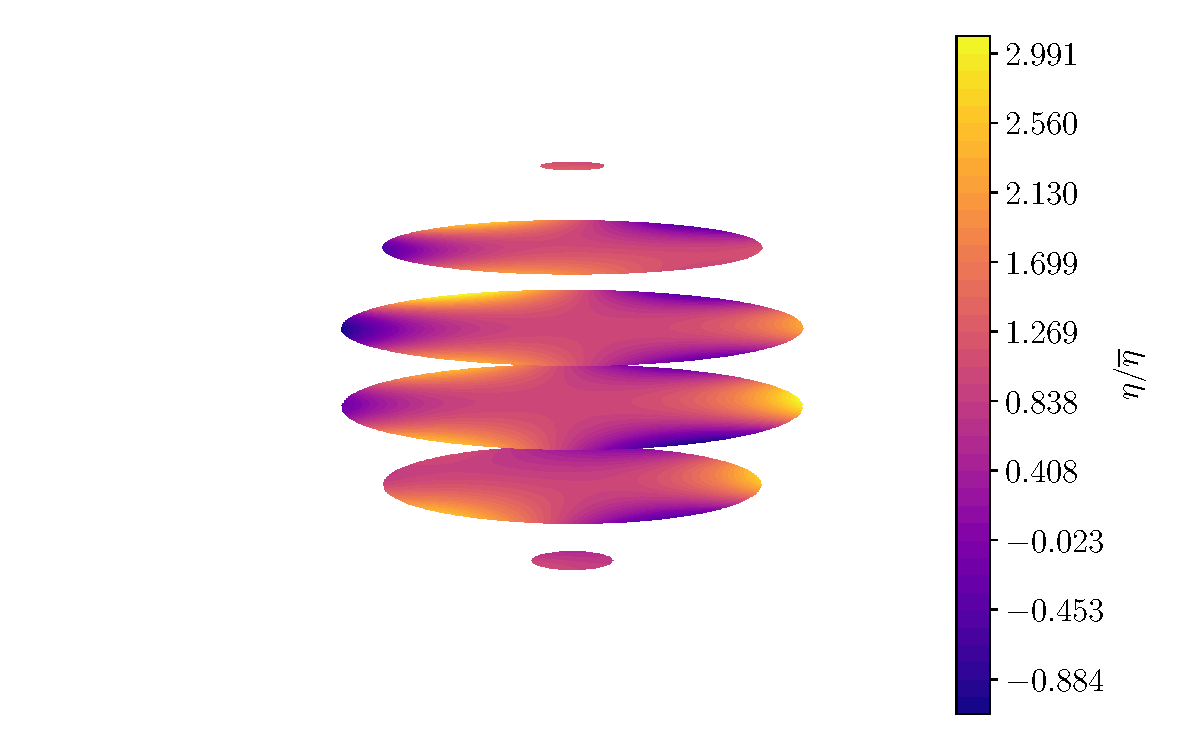
\includegraphics[width=0.45\textwidth]{figs/high-likelihood.pdf}
  \caption{\textit{Left}: the surface of a near-spherical asteroid with uniform density distribution extracted via the surface model. \textit{Right}: the density distribution extracted via the likelihood model for the same density moments but a spherical surface. The same length scale is used in both figures.}
  \label{fig:surface-density}
\end{figure*}

In section \ref{sec:density-distro}, we mention that the shape of the asteroid can be computed from observations of the density moments and $a_\mathcal{A}$ if a uniform density distribution is assumed. We did not further describe the model in the main text because it is unlike the other three models in the nature of its assumptions, and in the fact that it is non-linear. However, it may be a useful technique so it is mentioned here; we call it the ``surface'' model. A similar model was also studied in Ref.~\cite{BAXANSKY2007756}.

Suppose our asteroid has constant density $\rho_0$ and known parameters $K_{\ell m}$ and $a_\mathcal{A}^2$, and that the asteroid is ``star shaped'' in that every ray originating from the centre of mass of the asteroid (the origin of the body-fixed frame) passes through the surface of the asteroid exactly once, at distance $r(\theta, \phi)$ written in spherical coordinates. By the divergence theorem, we write
\begin{equation}
  K_{\ell m} = \frac{\rho_0}{\mu_\mathcal{A} a_\mathcal{A}^\ell} \oint_{\partial \mathcal{A}} d^2 \bm r \cdot \bm v (\bm r)
\end{equation}
where $\bm v (\bm r) = \unit r R_{\ell m} (\bm r) r / (3+\ell) $ so that $\nabla \cdot \bm v(\bm r) = R_{\ell m}(\bm r)$. The integral is carried out over the surface of the asteroid. We know the area element satisfies $d^2 \bm r = (\partial \bm r / \partial \theta \times \partial \bm r / \partial \phi) d\theta d\phi$ in our coordinates, and when dotted with $\bm v \parallel \unit r$, this gives
\begin{equation}
  K_{\ell m} = \frac{\rho_0 }{\mu_\mathcal{A} a_\mathcal{A}^\ell (3 + \ell)} \int d\Omega r(\theta, \phi)^3 R_{\ell m}(r(\theta, \phi), \theta, \phi).
  \label{eqn:surface-klm}
\end{equation}
where the integral is carried out over the unit sphere. Note that the integrand of each $K_{\ell m}$ is proportional to $r(\theta, \phi)^{(3+\ell)}$ times constants and a spherical harmonic.

We write 
\begin{equation}
  r(\theta, \phi) = \sum_{\ell m} Y_{\ell m}^* C_{\ell m}
\end{equation}
without loss of generality. To keep $r(\theta, \phi) \in \mathds{R}$, we require $C_{\ell m}^* = (-1)^m C_{l,-m} (\ell-m)!/(\ell+m)$. With this definition, equation \ref{eqn:surface-klm} becomes a polynomial of degree $3+\ell$ in terms of $C_{\ell m}$ and integrals of products of spherical harmonics. These integrals can be pre-computed so that equation \ref{eqn:surface-klm} can then be numerically solved via standard polynomial solution methods to find $C_{\ell m}$. A similar equation to equation \ref{eqn:surface-klm} can be written for $a_\mathcal{A}$
\begin{equation}
  a_\mathcal{A}^2 = \frac{\rho_0}{5\mu_\mathcal{A}}\int d\Omega r(\theta, \phi)^5
  \label{eqn:surface-am}
\end{equation}
which can also be solved via polynomial methods.

Equations \ref{eqn:surface-klm} and \ref{eqn:surface-am} form $(\ell_\text{max} + 1)^2 + 1$ constraints, where $\ell_\text{max}$ is the maximum degree of $C_{\ell m}$. By setting the same maximum degree as for the known $K_{\ell m}$, the system is well-determined and will yield finitely many solutions. These solutions can be filtered by removing those that produce $r(\theta, \phi) < 0$ for any $\theta, \phi$, which is unphysical.

To test the model, this process was run for an asteroid with $K_{1m}=K_{2m'}=0$, but randomly chosen $K_{3m}$ in the range 0.01 to -0.01. The resulting surface is shown in figure \ref{fig:surface-density}. The figure shows a near-spherical asteroid, which is expected for $K_{\ell m} = 0$ for $\ell > 0$. However, the additional $K_{3m}$ components clearly induce non-sphericity in the asteroid which is captured by the surface model.

To give an alternate view of the non-sphericities found via this new surface model, figure \ref{fig:surface-density} also displays the density distribution extracted via the likelihood model assuming a spherical asteroid shape, but with the same density moments. (Uncertainty in the moments is not modelled in this figure, to better compare the two.) Where the likelihood model displays low density, the surface model clearly retracts into the asteroid. Where the likelihood model yields high density, the surface model extends. Thus, the connection made in section \ref{sec:spherical-density} between non-uniformities in extracted densities at the asteroid surface and inaccuracies in the surface shape is more firmly represented.

This surface model could, in principle, be used to improve estimates of the surface of an asteroid made by light curve analysis, since it connects rotational data to the asteroid surface which reflects the light we observe. Thus, uncertainties either in the density moments or the asteroid surface (or both), could be reduced. However, light-curve analysis is beyond the scope of this paper.

